Once we established our plan, we started dwelving into the details of our optimization. Our method is based on the idea that looking at recent performance of strategies can be a good method to assign weights. So we believe that if a strategy has had a good Sharpe-Ratio over the last two months the strategy is working well and mught be worth putting it in production allocating a significant portion of risk to it. (Un)fortunately, systematic risk must also be taken into account, therefore we elaborate a method to apply this logic within a sharpe-based allocation framework, without looking a pure correlations.\\
As outlined before, the first step is to cluster the strategies. For this purpose we need to find an algorithm that fulfills our need. We decided to go for the \textit{Affinity Propagation} algorithm. This has the huge advantage that doesn't require us to set the number of clusters that are generated. Therefore requires no tuning. It's also much better because every week we have a different number of strategies to be put into production, so we cannot a priori know which is the best number of clusters to create.\\
To perform this clustering we need some preprocessing upfront, in fact we need to put the data in a way that it is understandable for our clustering algorithm. We remove outliers from the PnL series and standardize the data. At this point we face two choices: either computing a covariance matrix and feed it into the Affinity Propagation, or we simply reduce some noise through a PCA from the PnL Serieses and cluster them directly. The second idea sounds more interesting for two main reasons: first, we have many strategies and not many data points and computing a large covariance matrix in such case will be inefficient and error prone. On the other hand the PCA offers very stable and robust results. To perform the PCA we need to assess the ideal number of features to keep, and here we look for a sweet spot in the trade-off between number of PCA components and total explained variance.\\
To do so we draw a simple chart:

\begin{center}
	\centering
	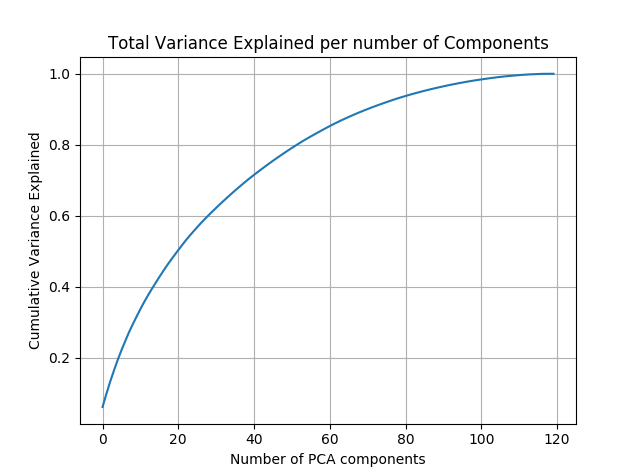
\includegraphics[width=0.6\textwidth]{HRP/PCA_Components.png}
	\captionof{figure}{Variance Explained by number of PCA components}
	\label{CRP_PCA}
\end{center}

We can see how the ideal number of features is about 80, with such a number of components we don't miss too much information and we can still run the code efficiently. With 80 features we explain roughly 95\% of the total variance, that is a very good result.\\
Now we can directly apply the clustering algorithm to these reduced data. This will allow us to come up with several clusters. Each cluster will then be assigned a weight of 1/Total number of clusters.\\
The last part is to assign weights within each cluster based on past Sharpe ratio. To do so, we need a certain window in the past and this is a number on which we will optimize the whole portfolio. In this part we will look at recent windows in the range of 20-120 trading days.\\ 

